%=====================================================================
%  FINAL SHORT REPORT
%  Autonomous TEC-Based Atmospheric-Water PV-Cleaning Robot
%
%  Project : Graduation Project (REE598/REE599)
%  Author  : Rahma El-Hamouly
%  Units   : SI (siunitx) | Citations: IEEE (IEEEtran.bst)
%
%  All numerical values are taken from the verified calculation and
%  simulation engine scripts/tec_robot_design.py, archived in
%  output/tec_robot_results.json, and from output/calculation_summary.txt
%  (Benban feasibility study).
%=====================================================================
\documentclass[11pt,a4paper]{article}

\usepackage[utf8]{inputenc}
\usepackage[T1]{fontenc}
\usepackage{lmodern}
\usepackage[english]{babel}

\usepackage{amsmath,amssymb}
\usepackage{mathtools}
\usepackage{siunitx}
\sisetup{per-mode=symbol,detect-all}
\DeclareSIUnit{\year}{yr}
\DeclareSIUnit{\dy}{day}
\DeclareSIUnit{\kWh}{kWh}
\DeclareSIUnit{\Wh}{Wh}
\DeclareSIUnit{\liter}{L}

\usepackage{graphicx}
\usepackage{float}
\usepackage{booktabs}
\usepackage{caption}
\usepackage{subcaption}

\usepackage[margin=2.5cm]{geometry}
\usepackage{setspace}
\onehalfspacing
\usepackage{cite}
\usepackage[colorlinks=true,linkcolor=blue,citecolor=blue,urlcolor=blue]{hyperref}

\newcommand{\degC}{\si{\degreeCelsius}}
\newcommand{\Wp}{W\textsubscript{p}}

\title{\bfseries Autonomous Thermoelectric Atmospheric-Water\\
Photovoltaic-Cleaning Robot\\[0.4em]
\large Final Short Report --- Design, Simulation, and Feasibility Summary}
\author{Rahma El-Hamouly\\ \small Graduation Project (REE598), Faculty of Engineering}
\date{June 2026}

\begin{document}
\maketitle

%=====================================================================
\begin{abstract}
\noindent
This project designs an autonomous robot that cleans photovoltaic (PV)
panels with distilled water it condenses from the night air using
thermoelectric (TEC) coolers, removing the trucked-water logistics that
make wet cleaning expensive in Egypt's deserts. The design targets three
deployment scales in Egypt's new sustainable cities: commercial rooftops,
residential rooftops, and street-lamp PV. The condenser is built from the
Egyptian-market TEC1-12706 module (\num{130}~EGP $\approx$ \num{2.71}~USD;
extracted coefficients $\alpha=\SI{0.0513}{\volt\per\kelvin}$,
$R=\SI{2.00}{\ohm}$, $K=\SI{0.546}{\watt\per\kelvin}$,
$Q_{c,\max}=\SI{56.4}{\watt}$). Simulated over \num{8784} hourly Benban
climate records, one tile yields \SI{5.35}{\liter\per\year}
(\SI{14.65}{\gram\per\dy}) for \SI{22.25}{\kWh\per\year} at a mean COP of
\num{1.44} under a smart night-only strategy with a \SI{5}{\kelvin}
condensation margin. A 69-tile array meets the \SI{1}{\liter\per\dy}
target (\SI{1.011}{\liter\per\dy}, \SI{369}{\liter\per\year}) at a
specific energy consumption of \SI{4.16}{\kWh\per\liter} thermoelectric,
\SI{5.27}{\kWh\per\liter} with parasitics. The system draws
\SI{5.32}{\kWh\per\dy} (TEC \SI{79}{\percent}, fans \SI{20}{\percent}),
requiring \num{1147}~\Wp{} of dedicated PV and a
\SI{698}{\ampere\hour}, \SI{12}{\volt} battery at the old
\SI{1.8}{\liter\per\square\meter} wet-wash dose. The microfibre robot cleans at
\SI{0.3}{\liter\per\square\meter}, a sixfold cut that makes full water self-supply
feasible: at the NAC reference site, 38 TEC tiles drawing about
\SI{14}{\percent} of the host array's energy meet the entire cleaning
demand, with one robot per array and a reservoir to bridge seasonal yield
swings. A 4-tile bench prototype
($\approx$\,\SI{59}{\gram\per\dy} expected, $\approx$\,\num{5760}~EGP) is
specified to validate the per-tile physics.
\end{abstract}

%=====================================================================
\section{Introduction and motivation}
\label{sec:intro}

Dust soiling costs PV plants in arid climates \SIrange{20}{30}{\percent}
of annual energy if panels are left
uncleaned~\cite{kazem2023soiling,sarver2013pvsoiling,caron2013soiling},
with arid-site soiling rates of \SIrange{0.3}{0.8}{\percent\per\dy}.
Wet cleaning restores this energy effectively, and condensate-based
cleaning has been measured to recover up to \SI{14}{\percent} of PV
output~\cite{shah2023condensate}, but it consumes water that must be
trucked into the desert, an expensive and scarce
resource~\cite{mejia2021cleaning}. The two problems compound in Egypt's
new sustainable cities (New Administrative Capital, New Alamein, New
Mansoura), where Vision 2030 plans distribute PV across commercial
rooftops, residential rooftops, and solar street
lights~\cite{egypt2030vision}: thousands of small, dispersed arrays that
no water truck route serves economically.

The project answers this with a robot that makes its own cleaning water.
A thermoelectric (Peltier) condenser cools a plate below the night-time
dew point, collects distilled condensate, and a brush-and-spray head
applies it to the panel. The water is effectively distilled
(conductivity below \SI{10}{\micro\siemens\per\centi\meter}), so it
leaves no mineral streaking, and the unit runs unattended on its own PV
and battery. The design covers three platform variants: a rooftop
rail-guided carriage for commercial arrays (\SIrange{50}{500}{\kilo\watt} scale), a
lighter carriage for residential arrays (\SIrange{3}{20}{\kilo\watt}), and
a pole-mounted unit for street-lamp panels
(\SIrange{100}{400}{\watt})~\cite{mohammed2021streetlamp}.

%=====================================================================
\section{Project evolution}
\label{sec:evolution}

The project began as a utility-scale study: sizing atmospheric water
harvesting (AWH) plant to supply cleaning water for a
\SI{200}{\mega\watt} block of the Benban Solar Park (Aswan,
\ang{24.45}\,N, \ang{32.75}\,E)~\cite{benban_irena}. That study computed
an annual cleaning-water duty of \SI{37674}{\cubic\meter\per\year} and
compared AWH routes by levelised cost of water
(LCOW)~\cite{kim2022lcow,bagheri2024sec}: vapour-compression
refrigeration (VCR) at \SI{13.98}{USD\per\cubic\meter}, absorption at
\SI{13.18}{USD\per\cubic\meter}, and TEC at
\SIrange{44.96}{244.96}{USD\per\cubic\meter} depending on the assumed
specific energy consumption.

On 24 April 2026 the project pivoted. The Benban numbers showed that TEC
condensation cannot compete with VCR at utility scale, but they also
proved the physics works: atmospheric water harvesting is viable in the
arid Egyptian climate (relative humidity \SIrange{25}{55}{\percent},
ambient \SIrange{25}{42}{\degreeCelsius}), and TEC modules reach the
required dew-point temperatures with hardware cheap and small enough to
ride on a robot. At robot scale the comparison inverts: a VCR compressor
loop is too heavy and maintenance-bound for an \SI{8}{\kilogram} mobile
platform, while TEC tiles are solid-state, modular, and cost
\num{130}~EGP each on the Egyptian market. The Benban work is therefore
retained as feasibility evidence in the methodology, and the autonomous
robot is the deliverable.

%=====================================================================
\section{System design summary}
\label{sec:design}

\subsection{TEC atmospheric water generator module}

The condenser tile is the TEC1-12706, the most widely stocked Peltier
module in Egypt. Its catalogue maxima
($I_{\max}=\SI{6.0}{\ampere}$, $U_{\max}=\SI{15.4}{\volt}$,
$\Delta T_{\max}=\SI{66}{\kelvin}$) convert to the device coefficients
$\alpha=\SI{0.0513}{\volt\per\kelvin}$, $R=\SI{2.00}{\ohm}$, and
$K=\SI{0.546}{\watt\per\kelvin}$ through the standard maximum-parameter
relations~\cite{zhao2022teccondenser,riffat2003peltier}; the implied
$Q_{c,\max}=\SI{56.4}{\watt}$ falls inside the catalogue band of
\SIrange{50}{57}{\watt}, confirming the extraction. The operating point
couples the thermoelectric heat balance
\begin{equation}
  Q_C = \alpha I T_C - \tfrac{1}{2}I^2 R - K(T_H - T_C),
  \qquad \mathrm{COP} = \frac{Q_C}{\alpha I (T_H-T_C) + I^2 R},
  \label{eq:tec}
\end{equation}
to the condensation mass flux on the cold plate, driven by the vapour
density difference between the bulk air and the saturated layer at the
plate~\cite{eslami2021tec,shourideh2021tec}:
\begin{equation}
  \dot m = h_m A_c \left[\rho_v(T_{air},RH) - \rho_{v,sat}(T_C)\right],
  \label{eq:mdot}
\end{equation}
with $h_m=\SI{0.0235}{\meter\per\second}$ from the Lewis analogy at a
\SI{2}{\meter\per\second} fan-driven face velocity. The controller holds
the plate \SI{5}{\kelvin} below the dew point (the condensation margin
that maximises annual yield) and harvests only during hours when this
set-point is reachable within $I_{\max}$, the ``smart'' strategy. This
raises the mean COP from \num{0.78} (all-night operation) to \num{1.44}
and cuts specific energy consumption by \SI{78}{\percent} at the cost of
\SI{34}{\percent} of the water. One tile then delivers
\SI{5.35}{\liter\per\year} (\SI{14.65}{\gram\per\dy}) for
\SI{22.25}{\kWh\per\year}; \num{69} tiles meet the
\SI{1}{\liter\per\dy} design target.

\subsection{Water handling}

Condensate runs off the anodised aluminium cold plate, tilted \ang{15},
into a gutter and a reservoir with a level switch. A frost floor
protects the winter operating points, where Benban dew points approach
\SI{0}{\degreeCelsius}:
\begin{equation}
  T_{C,set} = \max\!\left(T_{dew} - \SI{5}{\kelvin},\; \SI{1}{\degreeCelsius}\right).
  \label{eq:frost}
\end{equation}
A \SI{12}{\volt} diaphragm micro-pump feeds the spray bar at the brush.
Each cleaning event uses \SI{0.6}{\liter}
(\SI{0.3}{\liter\per\square\meter}, the microfibre dose within the
\SIrange{0.1}{0.5}{\liter\per\square\meter} band for water-assisted robotic
PV cleaning), and the simulated annual yield supports
\num{102.5} events per year, one cleaning every three to four days,
which matches the arid-site soiling rate~\cite{kazem2023soiling}.

\subsection{Chassis and drive}

The platform is an \SI{8}{\kilogram} rail-guided carriage that rides
guide rails on panels inclined up to \ang{24}; a free differential-drive
crawler could not hold yaw on \ang{24} glass in simulation, so the drive
was constrained to the rail. A rack-and-pinion moves the carriage along
the fall line. The resistive force on the slope, gravity plus rolling
resistance~\cite{siegwart2011mobilerobots}, is
\begin{equation}
  F_{resist} = mg\sin\beta + \mu_{roll}\, mg\cos\beta = \SI{42.7}{\newton},
  \label{eq:fresist}
\end{equation}
which at a \SI{0.030}{\meter} pinion (\SI{0.015}{\meter} pitch radius) sets a
required pinion torque of $F_{resist}\,r_p \approx \SI{0.64}{\newton\meter}$,
raised to at least \SI{0.84}{\newton\meter} once the 1.5 safety factor and
drivetrain losses are carried. The drive runs near \SI{38}{rpm} to give the
\SI{0.06}{\meter\per\second} sweep speed.

\subsection{Cleaning head}

A full-width \SI{0.96}{\meter} soft brush (\SI{50}{\milli\meter} diameter)
spans the panel, so the carriage cleans in one fall-line sweep rather than a
multi-pass path: a single down-and-up traverse takes \SI{66.7}{\second} per
\SI{2}{\square\meter} panel at \SI{0.06}{\meter\per\second}. Cleaning
energy is negligible in the budget because events are short and
infrequent.

\subsection{Power and battery}

Table~\ref{tab:energy} gives the annual-mean daily budget of the full
69-tile system. The TEC stack dominates at \SI{79}{\percent}; the
\num{36} cold- and hot-side fans add \SI{20}{\percent}; everything
else, the controller and the cleaning actuators, is about
\SI{1}{\percent}. With a Benban peak-sun-hour figure of
\SI{5.8}{\hour\per\dy} and a performance ratio of
\num{0.80}~\cite{nasa_power,globalsolaratlas}, the supply sizing is
\begin{equation}
  P_{pv} = \frac{E_{total}}{PSH \cdot PR} = \num{1147}~\text{\Wp}
  \;(\approx \SI{5.34}{\square\meter}),
  \qquad
  C_{batt} = \frac{E_{store}\,k_{margin}}{V_{batt}\, DoD\, \eta_{chg}}
  = \SI{698}{\ampere\hour}~\text{at}~\SI{12}{\volt},
  \label{eq:supply}
\end{equation}
i.e.\ an \SI{8.4}{\kWh} LiFePO$_4$ store for one night of autonomy at
\SI{80}{\percent} depth of discharge. Because harvesting follows the
humid months, the demand is strongly seasonal
(Fig.~\ref{fig:energybal}); the array is sized to the annual-mean load
and the \SI{20}{\percent} design margin is carried by the energy store
rather than the array.

\begin{table}[H]
  \centering
  \caption{Daily energy budget of the full-scale system (smart strategy).}
  \label{tab:energy}
  \begin{tabular}{lc}
    \toprule
    \textbf{Load} & \textbf{Energy (\si{\Wh\per\dy})}\\
    \midrule
    TEC stack (69 tiles)     & 4205.9\\
    Fans (36)                & 1080.0\\
    MCU + sensors            & 36.0\\
    Cleaning (motors + pump) & 0.9\\
    \midrule
    \textbf{Total}           & \textbf{5322.8} ($=\SI{5.32}{\kWh\per\dy}$)\\
    \bottomrule
  \end{tabular}
\end{table}

\begin{figure}[H]
  \centering
  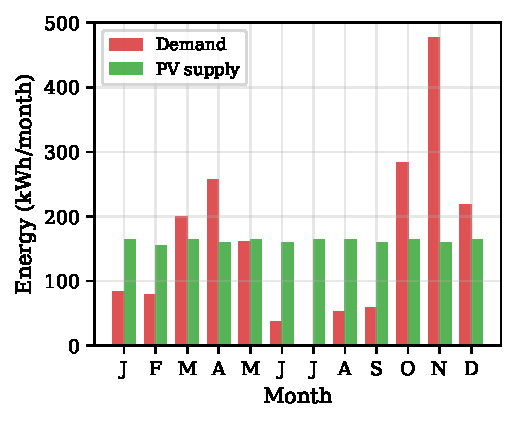
\includegraphics[width=0.58\textwidth]{figures/fig_energy_balance.pdf}
  \caption{Monthly energy demand of the 69-tile system against the output
           of the \num{1147}-\Wp{} array sized to the annual-mean load.
           Harvesting demand concentrates in the humid winter months.}
  \label{fig:energybal}
\end{figure}

\subsection{Control and autonomy}

A finite-state supervisor runs on an ESP32-class microcontroller:
\textsc{Idle} $\rightarrow$ \textsc{Harvest} (night, set-point
reachable) $\rightarrow$ \textsc{Store} $\rightarrow$ \textsc{Clean}
(reservoir $\geq$ \SI{0.6}{\liter} and soiling threshold reached)
$\rightarrow$ \textsc{Dock/Charge}. A temperature/humidity sensor feeds
the on-board dew-point computation; the cold plate tracks the
set-point~\eqref{eq:frost} through a discrete PID loop on the TEC
current (PWM) with anti-windup clamping at
$I_{\max}=\SI{6}{\ampere}$~\cite{shourideh2021tec}. Safety hardware
includes motor over-current cutouts, edge limit switches with
interrupt-driven reversal, an IMU tilt trip, and a watchdog timer.

%=====================================================================
\section{Simulation results}
\label{sec:sim}

The verified engine \texttt{tec\_robot\_design.py} evaluates the coupled
psychrometric and thermoelectric model over all \num{8784} hourly
records of air temperature and relative humidity for Benban in 2020
(NASA POWER~\cite{nasa_power}), restricted to night hours
(18:00--06:00). Figure~\ref{fig:climatepair} shows the climate input:
the dew point peaks in the cool, humid winter and collapses in summer,
and this, not air temperature, drives the yield.

\begin{figure}[H]
  \centering
  \begin{subfigure}[b]{0.48\textwidth}
    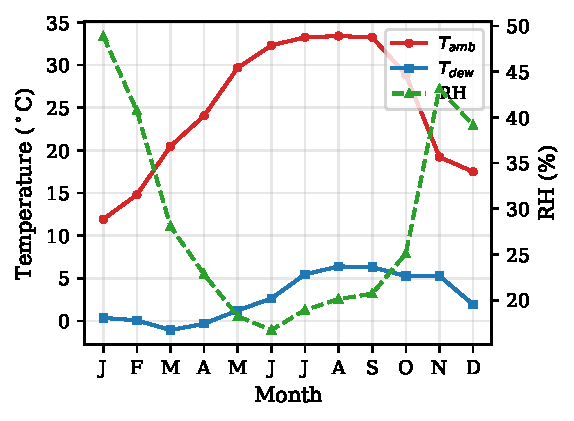
\includegraphics[width=\textwidth]{figures/fig_monthly_climate.pdf}
    \caption{Monthly mean $T$, $RH$, and dew point.}
  \end{subfigure}\hfill
  \begin{subfigure}[b]{0.48\textwidth}
    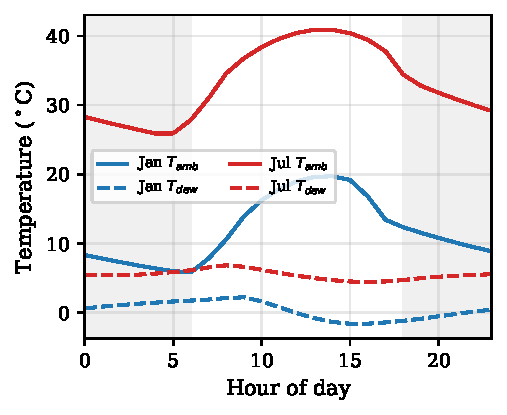
\includegraphics[width=\textwidth]{figures/fig_diurnal.pdf}
    \caption{Mean diurnal temperature and humidity.}
  \end{subfigure}
  \caption{Benban climate inputs (NASA POWER, 2020).}
  \label{fig:climatepair}
\end{figure}

Table~\ref{tab:monthly} and Fig.~\ref{fig:perfpair} summarise the
monthly behaviour of the 69-tile system. From October to March the
system exceeds its \SI{1}{\liter\per\dy} target, peaking at
\SI{4.5}{\liter\per\dy} in November. From June to September it produces
almost nothing: night dew points sit near \SI{6}{\degreeCelsius} at very
low humidity, the required temperature lift grows, and the COP falls
below \num{0.5} while the specific energy consumption climbs steeply.
The annual totals are \SI{369}{\liter} of water for
\SI{1942}{\kWh} of demand, i.e.\ \SI{4.16}{\kWh\per\liter} for the
thermoelectric stack alone and \SI{5.27}{\kWh\per\liter} for the full
system. These values sit inside the published experimental range of
\SIrange{2.8}{12}{\kWh\per\liter} for Peltier AWGs in hot, dry
air~\cite{shourideh2021tec,bagheri2024sec}, unlike an earlier proposal
figure discussed in Section~\ref{sec:status}.

\begin{table}[H]
  \centering
  \caption{Monthly simulation summary for the full-scale system (69 tiles).}
  \label{tab:monthly}
  \begin{tabular}{cccccc}
    \toprule
    \textbf{Month} & $T$ (\degC) & $RH$ (\si{\percent}) & $T_{dew}$ (\degC)
      & \textbf{Water} (\si{\liter\per\dy}) & \textbf{COP}\\
    \midrule
    Jan & 11.9 & 48.9 & 0.4  & 0.85 & 2.92\\
    Feb & 14.8 & 40.7 & 0.1  & 0.80 & 2.37\\
    Mar & 20.5 & 28.1 & $-1.1$ & 1.13 & 1.22\\
    Apr & 24.1 & 22.8 & $-0.3$ & 0.70 & 0.82\\
    May & 29.7 & 18.3 & 1.2  & 0.44 & 0.69\\
    Jun & 32.3 & 16.7 & 2.6  & 0.00 & 0.43\\
    Jul & 33.3 & 18.9 & 5.5  & n/a  & n/a\\
    Aug & 33.4 & 20.1 & 6.4  & 0.09 & 0.46\\
    Sep & 33.3 & 20.7 & 6.3  & 0.13 & 0.48\\
    Oct & 28.9 & 25.1 & 5.3  & 1.40 & 0.65\\
    Nov & 19.2 & 43.1 & 5.3  & 4.52 & 1.20\\
    Dec & 17.5 & 39.2 & 1.9  & 2.06 & 1.47\\
    \bottomrule
  \end{tabular}
\end{table}

\begin{figure}[H]
  \centering
  \begin{subfigure}[b]{0.48\textwidth}
    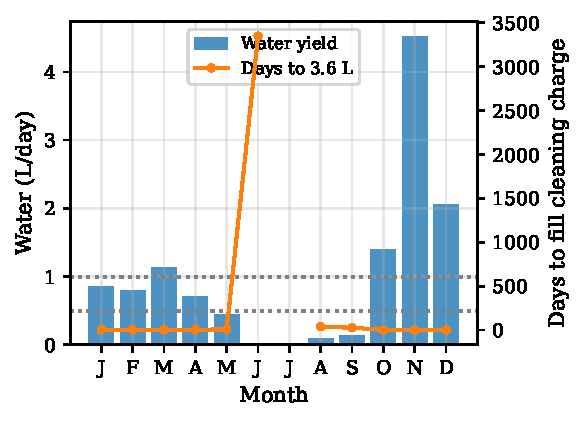
\includegraphics[width=\textwidth]{figures/fig_monthly_water.pdf}
    \caption{Monthly system water yield.}
  \end{subfigure}\hfill
  \begin{subfigure}[b]{0.48\textwidth}
    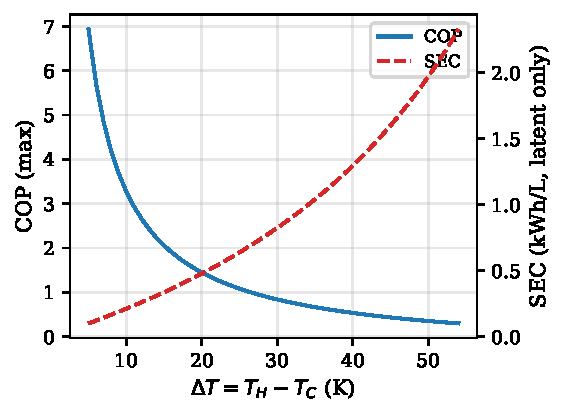
\includegraphics[width=\textwidth]{figures/fig_cop_sec_dT.pdf}
    \caption{COP and SEC vs.\ temperature lift.}
  \end{subfigure}
  \caption{Simulated performance. Yield tracks the dew point; COP falls
           and SEC rises as the required lift grows in summer.}
  \label{fig:perfpair}
\end{figure}

A sensitivity sweep of the condensation margin confirms the design
point: \SI{5}{\kelvin} maximises water yield
(\SI{5.35}{\liter\per\year} per tile) while \SI{8}{\kelvin} gives the
minimum SEC (\SI{4.09}{\kWh\per\liter}, \SI{2}{\percent} below the
design value). Water is the binding constraint, so the design takes
\SI{5}{\kelvin}.

%=====================================================================
\section{Feasibility conclusion}
\label{sec:feasibility}

The central finding concerns the cleaning water budget. The earlier
\SI{1.8}{\liter\per\square\meter} wet-wash dose put full self-sufficiency at
\SI{1}{\liter\per\dy}, costing \SI{5.32}{\kWh\per\dy} and
\SI{5.34}{\square\meter} of dedicated PV, more than the
\SI{2}{\square\meter} panel itself generates. The microfibre robot cleans
at \SI{0.3}{\liter\per\square\meter}, a sixfold cut, so full water self-supply is
feasible. At the NAC reference site, 38 TEC tiles draw
\SI{6.47}{\kWh\per\dy}, about \SI{14}{\percent} of the host array's energy,
to meet the entire \SI{1439}{\liter\per\year} demand (19 tiles and
\SI{7}{\percent} on a weekly schedule). Two design decisions follow:

\begin{enumerate}
  \item \textbf{One robot per array.} A shared dock harvests for the whole
        array, amortising the supply and AWG hardware over many panels. Drawn
        from the house array, the marginal AWG hardware is about
        \num{14000}~EGP.
  \item \textbf{Seasonal reservoir storage.} The harvester banks the
        October--March surplus in a reservoir to carry cleaning through the
        leaner summer months, so the supply stays on demand year round.
\end{enumerate}

This keeps the original goals, distilled water, no trucked-water
logistics, unattended operation, and the low-water microfibre dose closes
the cleaning loop on harvested atmospheric water.

%=====================================================================
\section{Current status and remaining work}
\label{sec:status}

\textbf{Completed.} Benban feasibility study (LCOW screening of five AWH
routes); verified per-tile TEC condensation model and annual hourly
simulation; full-scale sizing (tiles, fans, PV, battery); drive,
coverage-path, and cleaning-water sizing; control architecture; 4-tile
prototype specification, bill of materials
($\approx$\,\num{5760}~EGP~$\approx$~\num{120}~USD), and test plan with
uncertainty budget.

\textbf{Remaining.}
\begin{itemize}
  \item 3D CAD of the Scale-B (commercial rooftop) unit and the
        pole-mounted street-lamp variant.
  \item Reconciled full-system BOM with current Egyptian-market prices.
  \item Build and test the 4-tile bench prototype: expected yield
        $\approx$\,\SI{59}{\gram\per\dy}
        (\SIrange{40}{60}{\milli\liter} per favourable night),
        measurable on a \SI{0.1}{\gram} balance; validate per-tile
        yield, COP, and cleaning power recovery against the model.
\end{itemize}

The engineering review of the REE598 proposal
(\texttt{docs/REE598\_PROPOSAL\_REVIEW.md}) left eight numerical flags
open for author decision; they must be closed before REE599
fabrication:

\begin{enumerate}
  \item Tables 6.1 and 6.2 of the proposal disagree on annual energy
        recovered (Table 6.2 is 3.5--4.7$\times$ too high; corrected
        Scale-B payback is about 9 years, not 1.9).
  \item The proposal's TEC SEC of \SI{0.927}{\kWh\per\liter} is 3--10$\times$
        below published data; the present coupled solver
        (\SI{4.16}{\kWh\per\liter}) supersedes it and the proposal text
        needs updating.
  \item The hot-side temperature was treated as a free parameter; solving
        the Peltier and heat-sink equations together gives
        $T_h \approx \SI{50}{\degreeCelsius}$ and a lower COP.
  \item The claimed heat-sink resistance of \SI{0.5}{\kelvin\per\watt}
        is optimistic by 2--4$\times$ against datasheets for
        \SI{50}{\milli\meter} extrusions.
  \item The Scale-B BOM battery (\SI{1.8}{\kWh}) is \SI{25}{\percent}
        below the computed requirement (\SI{2.42}{\kWh}).
  \item The LiFePO$_4$ pack price in the BOM is below market; a
        realistic figure raises the Scale-B total to about \num{900}~USD.
  \item The Scale-C gantry with a 1.67-tonne water reservoir is
        structurally impractical; it should become a fleet of
        Scale-B-class units.
  \item At the corrected \SI{0.3}{\liter\per\square\meter} microfibre dose a
        full-array event needs \SI{13.8}{\liter}, so the Scale-B condensate
        tank (\SI{5}{\liter}) holds most of one event; a modest tank upsize or
        a refill between modules covers the balance.
\end{enumerate}

%=====================================================================
\section{Conclusions}
\label{sec:conclusions}

A robot that condenses its own distilled cleaning water from desert
night air is buildable from Egyptian-market parts: \num{69}
TEC1-12706 tiles at \num{130}~EGP each meet a \SI{1}{\liter\per\dy}
water target at a mean COP of \num{1.44} when operated only in
favourable night hours with a \SI{5}{\kelvin} condensation margin. The
energy price of that water, \SI{5.27}{\kWh\per\liter} at system level,
rules out a self-contained one-robot-per-panel loop and dictates the
architecture instead: one robot per array, with AWG harvesting as a
seasonal supply banked in a reservoir from the October--March surplus.
The Benban study that started the project survives as the climate
dataset and the proof that TEC condensation works in arid Egypt; the
4-tile bench prototype is the next step, and because the model is
per-tile linear, its measured yield validates the full-scale design
directly.

%=====================================================================
\bibliographystyle{IEEEtran}
\bibliography{references}

\end{document}
